\documentclass[aps,pra,10pt,nofootinbib]{revtex4}
%\pdfoutput=1
% Package(s) to include
%\listfiles
\usepackage{amsfonts,amssymb,amsmath}            % for math symbols.
\usepackage{lmodern,adjustbox}
\usepackage[skins,breakable]{tcolorbox}
\usepackage{tikz}
\usetikzlibrary{quantikz}
\tcbuselibrary{listings}
\tcbuselibrary{breakable}
\lstset{
basicstyle=\small\ttfamily,
columns=flexible,
breaklines=true
}
\usepackage[pdftex,hyperfigures,pdfpagelabels]{hyperref} 
%\lstloadlanguages{Latex}

\newtcolorbox{Code}{enhanced,fonttitle=\sffamily\bfseries\large,valign=center
,drop fuzzy shadow,sidebyside,lefthand ratio=0.4,lower separated=false}

\begin{document}

\title{Tutorial on the Quantikz Package}
\date{\today}
\author{Alastair \surname{Kay}}
\affiliation{Royal Holloway University of London, Egham, Surrey, TW20 0EX, UK}
\email{alastair.kay@rhul.ac.uk}
\begin{abstract}
\end{abstract}
\maketitle
I've always used \href{https://arxiv.org/abs/quant-ph/0406003}{QCircuit} for typesetting quantum circuit diagrams within \LaTeX, but found the Xy-pic based notation rather impenetrable and I struggled to adapt it for my needs (this is probably my failing rather than the package's). Thus, I wanted a tikz package that could do the same. That package is Quantikz. Those familiar with QCircuit will recognise much of the notation, although it has evolved a bit (hopefully simplified!).

\section{Usage}

The quantikz package is available on CTAN, and will therefore be available through most (current) TeX distributions. Once installed, simply write
\begin{verbatim}
\usepackage{tikz}
\usetikzlibrary{quantikz}
\end{verbatim}
in the preamble of your document
Now, each time that you want to include a quantum circuit, you just enclose it in a \verb!tikzcd! or \verb!quantikz! environment. (Theoretically, there is an advantange of \verb!quantikz! over \verb!tikzcd!, but \verb!tikzcd! is retained for backwards compatibility\footnote{\texttt{quantikz} should support the external package in tikz. I've never tried it.}.)

The current version of TeX on the arXiv is not up to date enough to provide the quantikz package. When uploading your source to the arXiv, you need to obtain the file tikzlibraryquantikz.code.tex (you will always be able to locate it on your computer in the main tex directory if you have installed the package, but it should also accompany the source code of this file, and the most recent version will is available \href{http://dx.doi.org/10.17637/rh.7000520}{here}). Just include the file in the main directory of your source code.
\section{A Single Wire}
%\expandafter\def\expandafter\mname\expandafter{\getrandomletter}
Quantum circuits are laid out with a matrix notation, with cells separated by \& (just like all matrices, tables etc.\ in \LaTeX). Here, we typeset a single quantum wire.
\begin{Code}
\begin{center}
\begin{quantikz}
\lstick{$\ket{0}$} & \phase{\alpha} & \gate{H} & \phase{\beta} & \gate{H} & \phase{\gamma} & \rstick{Arbitrary\\pure state}\qw
\end{quantikz}
\end{center}
\tcblower
\begin{lstlisting}
   \begin{quantikz}
   \lstick{\ket{0}} & \phase{\alpha} & \gate{H} 
	   & \phase{\beta} & \gate{H} & \phase{\gamma}
	   & \rstick{Arbitrary\\pure state}\qw
   \end{quantikz}
\end{lstlisting}
\end{Code}
Single-qubit gates take the form \verb!\gate{H}!, with any sequence of maths allowed in the argument\footnote{See Sec.\ \ref{sec:trouble} in case you need to use \& characters in the maths.}, or, for phase gates, \verb!\phase{phase}!. The first gate should be in the second column rather than the first (so that the preceding quantum wire has somewhere to go). You {\em can} put it in the first column, it just won't have an incoming wire. 

Text can be added at the start of a quantum wire using \verb!\lstick{}!, and at the end using \verb!\rstick{}!. These are not maths environments, but you can of course insert maths delimiters such as \$.
Notice that a multi-line \verb!lstick! or \verb!rstick! is trivial\footnote{The only issue is that the height of the label will not be taken into account in the vertical spacing of quantum wires. You may have to adjust this manually. See Section \ref{sec:align} for an example of how to achieve this.}.

\subsection{Measurements}

There are several measurement devices to choose from, and the measurement basis can be specified as the parameter:
\begin{Code}
\begin{center}
\begin{quantikz}
& \meter{0} && \meterD{1} & & \measuretab{\text{out}}& & \measure{\text{basis}}
\end{quantikz}
\end{center}
\tcblower
\begin{lstlisting}
\begin{quantikz}
& \meter{0} && \meterD{1} && \measuretab{\text{out}} && \measure{\text{basis}}
\end{quantikz}
\end{lstlisting}
\end{Code}
Thus, in our previous circuit:
\begin{Code}
\begin{center}
\begin{quantikz}
\lstick{\ket{0}} & \phase{\alpha} & \gate{H} & \phase{\beta} & \gate{H} & \phase{\gamma} & \meter{$\ket{\pm}$}
\end{quantikz}
\end{center}
\tcblower
\begin{lstlisting}
\begin{quantikz}
\lstick{\ket{0}} & \phase{\alpha} & \gate{H} & \phase{\beta} & \gate{H} & \phase{\gamma} & \meter{$\ket{\pm}$}
\end{quantikz}
\end{lstlisting}
\end{Code}

\subsection{Wires and Arrows}

There are a few bells and whistles: \verb!\qw! connects a quantum wire from the current cell back to the previous one. Most gates have this built in (\verb!\rstick! is the notable exception). Equally, sometimes you want a `do nothing' operation, and \verb!\qw! is perfect for that. Also, you can just insert text into a cell without boxing it (as you would for a gate). This can be useful for errors, and is achieved with \verb!\push{}!. 
\begin{Code}
\begin{center}
\begin{quantikz}
\lstick{$\ket{0}$\\initial state} & \qw & \push{X} & \qw & \rstick{$\ket{1}$} \qw
\end{quantikz}
\end{center}
\tcblower
\begin{lstlisting}
\begin{quantikz}
\lstick{$\ket{0}$\\initial state} & \qw & \push{X} & \qw & \rstick{$\ket{1}$} \qw
\end{quantikz}
\end{lstlisting}
\end{Code}
Since we have built quantikz on top of tikzcd, any of the standard arrow commands will work. For example, after a measurement, you might want to use an arrow to report a particular measurement outcome using \verb!\arrow[r]!. The \verb!r! conveys that the arrow should head one cell to the right. You can use combinations of up (u), down (d), left (l) and right as you wish. For more styling options, see the \href{http://mirrors.ctan.org/graphics/pgf/contrib/tikz-cd/tikz-cd-doc.pdf}{tikzcd manual}.
\begin{Code}
\begin{center}
\begin{quantikz}
\lstick{$\ket{0}$\\initial state} & \qw & \push{X} & \qw & \meter{0/1} \arrow[r] & \rstick{$\ket{1}$}
\end{quantikz}
\end{center}
\tcblower
\begin{lstlisting}
\begin{quantikz}
\lstick{$\ket{0}$\\initial state} & \qw & \push{X} & \qw & \meter{0/1} \arrow[r] & \rstick{$\ket{1}$}
\end{quantikz}
\end{lstlisting}
\end{Code}

One particularly common reason for wanting an arrow is to indicate that a qubit is not being measured. There is a \verb!\trash! command in this instance.
\begin{Code}
\begin{center}
\begin{quantikz}
\lstick{$\ket{0}$} & \gate{H} & \trash{\text{trash}}
\end{quantikz}
\end{center}
\tcblower
\begin{lstlisting}
\lstick{$\ket{0}$} & \gate{H} & \trash{\text{trash}}
\end{lstlisting}
\end{Code}


Sometimes, you may want to group a whole bunch of wires together. Use \verb!\qwbundle! instead of \verb!\qw!.
\begin{Code}
\begin{center}
\begin{quantikz}
\lstick{$\ket{0}^{\otimes n}$} &[2mm] \gate{H}\qwbundle{3} &  \qw
\end{quantikz}
\end{center}
\tcblower
\begin{lstlisting}
\begin{quantikz}
\lstick{$\ket{0}^{\otimes n}$} &[2mm] \gate{H}\qwbundle{3} & \qw
\end{quantikz}
\end{lstlisting}
\end{Code}
\noindent The size of the strike can be altered by issuing the commands \verb!\pgfkeyssetvalue{/quantikz/Strike Height}{new height}! and \verb!\pgfkeyssetvalue{/quantikz/Strike Width}{new width}!. I felt this example benefited from some additional spacing (of 2mm) on one column. For more spacing options, see Sec.\ \ref{sec:spacing}.

You can access an alternative form for the multi-qubit wire using the \verb!alternate! key:
\begin{Code}
\begin{center}
\begin{quantikz}
\lstick{$\ket{0}^{\otimes n}$} & \gate{H} \qwbundle[alternate]{}&  \qwbundle[alternate]{} 
\end{quantikz}
\end{center}
\tcblower
\begin{lstlisting}
\begin{quantikz}
\lstick{$\ket{0}^{\otimes n}$} & \gate{H} \qwbundle[alternate]{}& \qwbundle[alternate]{} 
\end{quantikz}
\end{lstlisting}
\end{Code}
\noindent The alternate version does not typically represent how many wires are supposed to be in the bundle. However, there is the \texttt{alternate=2} option if you only want 2 wires.


\section{Multiple Qubits}

New rows are started with \textbackslash\textbackslash. If the wires don't interact, then you proceed exactly as before. Naturally, there are several gates that induce interaction between wires: \verb!\ctrl{3}! makes a control-qubit (for controlled-not, controlled-phase, controlled-$U$, etc), where the target is 3 wires below. \verb!\octrl! is near-identical, except the control circle is open, as usually used to convey being controlled off $\ket{0}$ instead of $\ket{1}$. These will need to be matched with target commands. These could be normal gates or \verb!\targ{}! (controlled-not), \verb!\control{}! (controlled-phase), \verb!\ocontrol{}! (controlled-phase, controlled off $\ket{0}$). There is also a swap gate, \verb!\swap{2}!, with target \verb!\targX{}!\footnote{For a variant, see Sec.\ \ref{sec:boxing}.}. These can be combined to give multi-controlled gates.
\begin{Code}
\begin{center}
\begin{quantikz}
\lstick{$\ket{0}$} & \gate{H} & \ctrl{1} & \gate{U} & \ctrl{1} & \swap{2} & \ctrl{1} & \qw  \\
\lstick{$\ket{0}$} & \gate{H} & \targ{} & \octrl{-1} & \control{} & \qw & \octrl{1} & \qw \\
&&&&&\targX{} & \gate{U} & \qw
\end{quantikz}
\end{center}
\tcblower
\begin{lstlisting}
\begin{quantikz}
\lstick{$\ket{0}$} & \gate{H} & \ctrl{1} & \gate{U} & \ctrl{1} & \swap{2} & \ctrl{1} & \qw  \\
\lstick{$\ket{0}$} & \gate{H} & \targ{} & \octrl{-1} & \control{} & \qw & \octrl{1} & \qw \\
&&&&&\targX{} & \gate{U} & \qw
\end{quantikz}
\end{lstlisting}
\end{Code}

If you want a gate that is one control and several targets, you may need the command \verb!\vqw{1}! (vertical quantum wire) to create vertical connections, or possibly \verb!\vcw{1}! to create the classical version.

\begin{Code}
\begin{center}
\begin{quantikz}
& \targ{} & \gate{U} & \qw \\
& \ctrl{1} \vqw{-1} & \meter{} \vcw{-1} \\
& \targ{} & \qw
\end{quantikz}
\end{center}
\tcblower
\begin{lstlisting}
\begin{quantikz}
& \targ{} & \gate{U} & \qw \\
& \ctrl{1} \vqw{-1} & \meter{} \vcw{-1} \\
& \targ{} & \qw
\end{quantikz}
\end{lstlisting}
\end{Code}
If you want to use classical controls with both horizontal and vertical components, you can do the following.
\begin{Code}
\begin{center}
\begin{quantikz}
& \ctrl{1} & \qw & \gate{U} & \gate{V} \\
& \targ{} \vqw{1} & \meter{} & \cwbend{-1}  \\
& \targ{} & \meter{} & \cw & \cwbend{-2} &
\end{quantikz}
\end{center}
\tcblower
\begin{lstlisting}
\begin{quantikz}
& \ctrl{1} & \qw & \gate{U} & \gate{V} \\
& \targ{} \vqw{1} & \meter{} & \cwbend{-1} \\
& \targ{} & \meter{} & \cw & \cwbend{-2} &
\end{quantikz}
\end{lstlisting}
\end{Code}

Standard gate commands will typically work well with the alternate option for bundled quantum wires. However, when using the \texttt{alternate=2} option, you may need to disable to default wire using the \texttt{nwires} option, as described in Sec.\ \ref{sec:wires}. However, the control can look messy. To that end, we use the \texttt{ctrlbundle} command.
\begin{Code}
\begin{center}
\begin{quantikz}
\lstick{\ket{x}} & \ctrlbundle{1} & \rstick{\ket{x}}\qwbundle[alternate]{} \\
& \gate[nwires=1]{U_x}\qwbundle[alternate=2]{} & \qwbundle[alternate=2]{}
\end{quantikz}
\end{center}
\tcblower
\begin{lstlisting}
\begin{quantikz}
\lstick{\ket{x}} & \ctrlbundle{1} & \rstick{\ket{x}}\qwbundle[alternate]{} \\
& \gate[nwires=1]{U_x}\qwbundle[alternate=2]{} & \qwbundle[alternate=2]{}
\end{quantikz}
\end{lstlisting}
\end{Code}
If \texttt{ctrlbundle} should only use two wires, supply the optional parameter \texttt{[2]},
\begin{Code}
\begin{center}
\begin{quantikz}
\lstick{\ket{x}} & \ctrlbundle[2]{1} & \rstick{\ket{x}}\qwbundle[alternate=2]{} \\
& \gate{U_x}\qwbundle[alternate]{} & \qwbundle[alternate]{}
\end{quantikz}
\end{center}
\tcblower
\begin{lstlisting}
\begin{quantikz}
\lstick{\ket{x}} & \ctrlbundle[2]{1} & \rstick{\ket{x}}\qwbundle[alternate=2]{} \\
& \gate{U_x}\qwbundle[alternate]{} & \qwbundle[alternate]{}
\end{quantikz}
\end{lstlisting}
\end{Code}

\section{Operating on Many Qubits}

We have already met the \verb!\lstick!, \verb!\rstick!, and \verb!\gate! commands. By default, these all act on a single quantum wire. However, they also take the optional parameter \verb!wires=n! to specify that they should extend over $n$ wires. The syntax is otherwise unchanged\footnote{Strictly, the \texttt{wires=} statement should not be necessary, as this is presumed to be the default key, but it is useful for readability.}.

\begin{Code}
\begin{center}
\begin{quantikz}
\lstick[wires=3]{$\ket{0}^{\otimes 3}$} & \ctrl{1} & \meter{} \\
 & \gate[wires=2]{U} & \qw\rstick[wires=2]{$\ket{11}$} \\
 &  & \qw
\end{quantikz}
\end{center}
\tcblower
\begin{lstlisting}
\begin{quantikz}
\lstick[wires=3]{$\ket{0}^{\otimes 3}$} & \ctrl{1} & \meter{} \\
 & \gate[wires=2]{U} & \qw\rstick[wires=2]{$\ket{11}$} \\
 &  & \qw
\end{quantikz}
\end{lstlisting}
\end{Code}

If you want to add extra width on the \verb!\gate!, use the second optional parameter to specify a width (note that this is a minimum width -- if your supplied text is wider, the box will adjust its width accordingly.
\begin{Code}
\begin{center}
\begin{quantikz}
& \gate{H} & \ctrl{1} & \meter{} \\
& \gate[wires=2][2cm]{U}  & \targ{} & \qw \\
&  & \qw & \qw
\end{quantikz}
\end{center}
\tcblower
\begin{lstlisting}
\begin{quantikz}
& \gate{H} & \ctrl{1} & \meter{} \\
& \gate[wires=2][2cm]{U}  & \targ{} & \qw \\
&  & \qw & \qw
\end{quantikz}
\end{lstlisting}
\end{Code}
Often, it is nice to be able to label the inputs and outputs on the box, which we do with the \verb!\gateinput! and \verb!\gateoutput! commands. These commands take 1 compulsory argument -- the label text. By default, this applies to a single wire, but you can again use the optional \verb!wires! parameter to extend it. The starting point is determined by where the command is placed. The width of the gate does not automatically adjust to the contents of these extra labels, so you will have to add it with the second optional parameter of \verb!\gate!.
\begin{Code}
\begin{center}
\begin{quantikz}
&\ctrl{1} & \qw \\
&\gate[wires=3][1.7cm]{U}
	\gateinput[wires=2]{$x$}
	\gateoutput[wires=2]{$x$}
	&\qw \\
& & \qw \\
&\gateinput{$y$}
\gateoutput{$y\oplus f(x)$}
&\qw
\end{quantikz}
\end{center}
\tcblower
\begin{lstlisting}
\begin{quantikz}
&\ctrl{1} & \qw \\
&\gate[wires=3][1.7cm]{U}
	\gateinput[2]{$x$}
	\gateoutput[wires=2]{$x$}&\qw \\
& \qw & \qw \\
&\qw\gateinput{$y$}\gateoutput{$y\oplus f(x)$}&\qw
\end{quantikz}
\end{lstlisting}
\end{Code}

You can use standard \LaTeX maths expressions for your labels. Usually, spacing can be automatically adjusted just fine. For example,

\begin{Code}
\begin{center}
\begin{quantikz}
& \gate{\sqrt{Z}} & \gate[2]{\sqrt{\textsc{swap}}} & \meter{} \\
& \gate{X}  & & \qw
\end{quantikz}
\end{center}
\tcblower
\begin{lstlisting}
\begin{quantikz}
& \gate{\sqrt{Z}} & \gate[2]{\sqrt{\textsc{swap}}} & \meter{} \\
& \gate{X}  & & \qw
\end{quantikz}
\end{lstlisting}
\end{Code}

Sometimes, it might be that you want a multi-line label, and it should not be that each wire takes the height of those multiple lines. At this point, use the key \verb!disable auto height!. By default, each row will be assigned the height that a gate with label $U$ would be. This can be overridden by the third optional parameter of the gate command, if desired.

\begin{Code}
\begin{center}
\begin{quantikz}
\lstick{$c_0$} & \gate[3,disable auto height]{\begin{array}{c} \text{M} \\ \text{A} \\ \text{J} \end{array}} & \qw & \qw \\
\lstick{$c_1$} &  &  \gate[3,disable auto height]{\begin{array}{c} \text{M} \\ \text{A} \\ \text{J} \end{array}} & \qw \\
\lstick{$c_2$} &  &  & \qw \\
\lstick{$c_3$} & \qw &  & \qw
\end{quantikz}
\end{center}
\tcblower
\begin{lstlisting}
\begin{quantikz}
\lstick{$c_0$} & \gate[3,disable auto height]{\begin{array}{c} \text{M} \\ \text{A} \\ \text{J} \end{array}} & \qw & \qw \\
\lstick{$c_1$} &  &  \gate[3,disable auto height]{\begin{array}{c} \text{M} \\ \text{A} \\ \text{J} \end{array}} & \qw \\
\lstick{$c_2$} &  &  & \qw \\
\lstick{$c_3$} & \qw &  & \qw
\end{quantikz}
\end{lstlisting}
\end{Code}

\subsection{Different Connections}\label{sec:wires}

It is assumed that most of the time you want to connect your gates with quantum wires. However, it is possible to override that, and either use classical wires, an alternate wire bundle, or no wire. These appear as option keys for the gate command, each of which are a comma-separated list of incoming wires that should be altered.

\begin{Code}
\begin{center}
\begin{quantikz}
& \gate[5,cwires={2,4},nwires={3},bundle={5}]{U} & \qw \\
& & \cw \\
& & \qw \\
& & \cw \\
& & \qwbundle[alternate]{}
\end{quantikz}
\end{center}
\tcblower
\begin{lstlisting}
\begin{quantikz}
& \gate[5,cwires={2,4},nwires={3},bundle={5}]{U} & \qw \\
& & \cw \\
& & \qw \\
& & \cw \\
& & \qwbundle[alternate]{}
\end{quantikz}
\end{lstlisting}
\end{Code}

\section{Slicing}

It is often helpful to `slice' up a circuit for the sake of explaining it step by step. To do this, we provide the \verb!\slice{title}! command, which inserts a dashed vertical line after the column in which the command is added.
\begin{Code}
\begin{center}
\begin{quantikz}
& \gate{H}\slice{step}  & \ctrl{1} & \meter{} \\
& \qw       & \targ{} & \ctrl{1} & \gate{H} & \qw \\
& \qw & \qw & \targ{} & \qw & \qw
\end{quantikz}
\end{center}
\tcblower
\begin{lstlisting}
\begin{quantikz}
& \gate{H}\slice{step}  & \ctrl{1} & \meter{} \\
& \qw       & \targ{} & \ctrl{1} & \gate{H} & \qw \\
& \qw & \qw & \targ{} & \qw & \qw
\end{quantikz}
\end{lstlisting}
\end{Code}
You can also slice every step by using option \verb!slice all!, and the labels will be automatically numbered. This is likely to behave strangely unless you explicitly ensure that all rows have the same number of entries (i.e.\ short rows should have extra \& characters added).
\begin{Code}
\begin{center}
\begin{quantikz}[slice all]
& \gate{H} & \ctrl{1} & \meter{} && \\
& \qw       & \targ{} & \ctrl{1} & \gate{H} & \qw \\
& \qw & \qw & \targ{} & \qw & \qw
\end{quantikz}
\end{center}
\tcblower
\begin{lstlisting}
\begin{quantikz}[slice all]
& \gate{H}  & \ctrl{1} & \meter{} && \\
& \qw       & \targ{} & \ctrl{1} & \gate{H} & \qw \\
& \qw & \qw & \targ{} & \qw & \qw
\end{quantikz}
\end{lstlisting}
\end{Code}
If you need to adjust where the last slice is, use the optional parameter \verb!remove end slices!, which counts the number of columns fewer to add slices to. You can also change the title of each of the slices, by setting \verb!slice titles!. Include the macro \verb!\col! in your specification if you want to use the step number. Note, however, that the columns won't space themselves out to accommodate a very wide label. You can style the slicing lines with the \verb!slice style! key, and the labels with \verb!slice label style!. These can be used to rotate the labels and create a bit more space!
\begin{Code}
\begin{center}
\begin{quantikz}[slice all,remove end slices=1,slice titles=slice \col,slice style=blue,slice label style={inner sep=1pt,anchor=south west,rotate=40}]
& \gate{H} & \ctrl{1} & \meter{} && \\
& \qw       & \targ{} & \ctrl{1} & \gate{H} & \qw \\
& \qw & \qw & \targ{} & \qw & \qw
\end{quantikz}
\end{center}
\tcblower
\begin{lstlisting}
\begin{quantikz}[slice all,remove end slices=1,slice titles=slice \col,slice style=blue,slice label style={inner sep=1pt,anchor=south west,rotate=40}]
& \gate{H}  & \ctrl{1} & \meter{} && \\
& \qw       & \targ{} & \ctrl{1} & \gate{H} & \qw \\
& \qw & \qw & \targ{} & \qw & \qw
\end{quantikz}
\end{lstlisting}
\end{Code}
\noindent This also gives the possibility to alter spacing if it would otherwise be a bit too tight.
\begin{Code}
\begin{center}
\begin{quantikz}[slice all,slice style={shorten <=-0.1cm,shorten >=-0.1cm},slice label style={yshift=0.1cm}]
\lstick{$\ket{0}$} & \gate{H} & \phase{\varphi} & \gate{H} & \rstick{$\cos\frac{\varphi}{2}\ket{0}-i\sin\frac{\varphi}{2}\ket{1}$}\qw
\end{quantikz}
\end{center}
\tcblower
\begin{lstlisting}
\begin{quantikz}[slice all,slice style={shorten <=-0.1cm,shorten >=-0.1cm},slice label style={yshift=0.1cm}]
\lstick{$\ket{0}$} & \gate{H} & \phase{\varphi} & \gate{H} & \rstick{$\cos\frac{\varphi}{2}\ket{0}-i\sin\frac{\varphi}{2}\ket{1}$}\qw
\end{quantikz}
\end{lstlisting}
\end{Code}
\noindent If you get compile errors when trying to slice, check the last line of your matrix, and make sure it doesn't end in \textbackslash\textbackslash.

The \verb!vertical slice labels! key reorients the labels as below. 
\begin{Code}
\begin{center}
\begin{quantikz}[slice all,remove end slices=1,slice titles=slice \col,vertical slice labels]
& \gate{H} & \ctrl{1} & \meter{} && \\
& \qw       & \targ{} & \ctrl{1} & \gate{H} & \qw \\
& \qw & \qw & \targ{} & \qw & \qw
\end{quantikz}
\end{center}
\tcblower
\begin{lstlisting}
\begin{quantikz}[slice all,remove end slices=1,slice titles=slice \col,vertical slice labels]
& \gate{H}  & \ctrl{1} & \meter{} && \\
& \qw       & \targ{} & \ctrl{1} & \gate{H} & \qw \\
& \qw & \qw & \targ{} & \qw & \qw
\end{quantikz}
\end{lstlisting}
\end{Code}

\section{Spacing}\label{sec:spacing}

\subsection{Local Adjustment}

There are several different ways in which we can manipulate the spacing of a diagram. Adding space to an individual row or column can be done in the standard way of tables in LaTeX. Here we add 2cm of space to the column between the $H$ and $X$ gates, and 1cm of space between the top two rows.
\begin{Code}
\begin{center}
\begin{quantikz}
& \gate{H} &[2cm] \gate{X} & \gate{H} & \qw \\[1cm]
& \gate{X} & \gate{Z} & \gate{Z} &\qw \\
& \gate{X} & \gate{Z} & \gate{Z} & \qw
\end{quantikz}
\end{center}
\tcblower
\begin{lstlisting}
\begin{quantikz}
& \gate{H} &[2cm] \gate{X} & \gate{H} & \qw \\[1cm]
& \gate{X} & \gate{Z} & \gate{Z} & \qw \\
& \gate{X} & \gate{Z} & \gate{Z} & \qw
\end{quantikz}
\end{lstlisting}
\end{Code}
If you don't know how much space you need, but it should be determined by the size of some text, you can use \verb!\hphantom{}! (widens the gate, in a similar way to \verb!\gate[1cm]{}!) or \verb!\hphantomgate{}! (increases the length of a wire) for horizontal spacing, and \verb!\ghost{}! for vertical spacing.
\begin{Code}
\begin{center}
\begin{quantikz}
& \gate{X} \hphantom{very wide} & \gate{X} & \hphantomgate{wide}\qw & \gate{X}
\end{quantikz}
\end{center}
\tcblower
\begin{lstlisting}
\begin{quantikz}
 & \gate{X} \hphantom{very wide} & \gate{X} & \hphantomgate{wide}\qw & \gate{X}
\end{quantikz}
\end{lstlisting}
\end{Code} 

\subsection{Global Adjustment}

Standard tikz commands facilitate a global adjustment of row and column spacing. For example, a ridiculous horizontal spacing:
\begin{Code}
\begin{center}
\begin{quantikz}[column sep=1cm]
& \gate{H} & \phase{\beta} & \gate{H} & \qw
\end{quantikz}
\end{center}
\tcblower
\begin{lstlisting}
\begin{quantikz}[column sep=1cm]
& \gate{H} & \phase{\beta} & \gate{H} & \qw
\end{quantikz}
\end{lstlisting}
\end{Code}
This specifically adjusts the \emph{gap} between the rows and columns, not the distance between the centres of the rows and columns. Depending on what gates you have on each wire, the spacing may not be the same between each wire. Sometimes this is desirable, particularly if a gate in one particular row is much larger than anything in the other rows. At other times, it just makes your diagram look a little odd. For example, look at the gap between the top two wires and the bottom two wires:
\begin{Code}
\begin{center}
\begin{quantikz}[row sep=0.1cm]
& \gate{X} & \ctrl{1} & \gate{X} & \qw \\
& \qw & \control{} & \qw & \qw \\
& \gate{X} & \qw & \qw & \qw \\
& \gate{H} & \qw & \qw & \qw 

\end{quantikz}
\end{center}
\tcblower
\begin{lstlisting}
\begin{quantikz}[row sep=0.1cm]
& \gate{X} & \ctrl{1} & \gate{X} & \qw \\
& \qw & \control{} & \qw & \qw \\
& \gate{X} & \qw & \qw & \qw \\
& \gate{H} & \qw & \qw & \qw 
\end{quantikz}
\end{lstlisting}
\end{Code}
If you want to make sure that every quantum wire is equally spaced, do the following to \verb!row sep!:
\begin{Code}
\begin{center}
\begin{quantikz}[row sep={0.6cm,between origins}]
& \gate{X} & \ctrl{1} & \gate{X} & \qw \\
& \qw & \control{} & \qw & \qw \\
& \gate{X} & \qw & \qw & \qw \\
& \gate{H} & \qw & \qw & \qw 

\end{quantikz}
\end{center}
\tcblower
\begin{lstlisting}
\begin{quantikz}[row sep={0.6cm,between origins}]
& \gate{X} & \ctrl{1} & \gate{X} & \qw \\
& \qw & \control{} & \qw & \qw \\
& \gate{X} & \qw & \qw & \qw \\
& \gate{H} & \qw & \qw & \qw 
\end{quantikz}
\end{lstlisting}
\end{Code}
This is particularly useful to achieve alignment of several circuits, as in \ref{sec:align}.

\subsection{Alignment}\label{sec:align}

How do we centre a circuit diagram? Simply surround it with \verb!\begin{center}! and \verb!\end{center}! commands, or within any standard equation environment.

Vertical alignment between different circuits can be more fiddly, depending on how much of a perfectionist you are. Sometimes, they work immediately, but the wires don't always align perfectly with each other. Generally the problem is that the highest gate in each row is different (here, the LHS is missing an $X$ gate on the second row)
\begin{Code}
\begin{center}
\begin{quantikz}
& \gate{X} & \ctrl{1} & \qw \\
& \qw & \targ{} & \qw
\end{quantikz}
\begin{quantikz}=\end{quantikz}\begin{quantikz}
& \ctrl{1} & \gate{X} & \qw \\
& \targ{}  & \gate{X} & \qw
\end{quantikz}
\end{center}
\tcblower
\begin{lstlisting}
\begin{quantikz}
& \gate{X} & \ctrl{1} & \qw \\
& \qw & \targ{} & \qw
\end{quantikz}
=\begin{quantikz}
& \ctrl{1} & \gate{X} & \qw \\
& \targ{}  & \gate{X} & \qw
\end{quantikz}
\end{lstlisting}
\end{Code}
\noindent  Ensuring an even spacing between rows, as described in Sec.\ \ref{sec:spacing}, can help (but is not always appropriate). Often the easiest is to fudge it using the \verb!\ghost! command which will add a 0-width gate of the height corresponding to its argument. So, having identified the problem with the above circuit, we can replace it with:
\begin{Code}
$$
\begin{quantikz}
& \gate{X} & \ctrl{1} & \qw \\
& \ghost{X}\qw & \targ{} & \qw
\end{quantikz}
=\begin{quantikz}
& \ctrl{1} & \gate{X} & \qw \\
& \targ{}  & \gate{X} & \qw
\end{quantikz}
$$
\tcblower
\begin{lstlisting}
\begin{quantikz}
& \gate{X} & \ctrl{1} & \qw \\
& \ghost{X}\qw & \targ{} & \qw
\end{quantikz}
=\begin{quantikz}
& \ctrl{1} & \gate{X} & \qw \\
& \targ{}  & \gate{X} & \qw
\end{quantikz}
\end{lstlisting}
\end{Code}

If you cannot identify the offending gate, and particularly if the operation is not a standard \verb!\gate! command, you might be better off combining the two circuits in a single circuit with no wires joining the two parts. The spacing works better if your circuit has an odd number of wires, otherwise you have to add an extra row in the middle, and then change the spacing of that row with its neighbours.
\begin{Code}
\begin{center}
\begin{quantikz}
& \qw & \ctrl{2} & \qw&&& \ctrl{2} & \gate{Z} & \qw \\[-0.3cm]
&&&&=&\\[-0.3cm]
& \gate{Z} & \targ{} & \qw&&& \targ{}  & \gate{Z} & \qw
\end{quantikz}
\end{center}
\tcblower
\begin{lstlisting}
\begin{quantikz}
& \qw & \ctrl{2} & \qw&&& \ctrl{2} & \gate{Z} & \qw \\[-0.3cm]
&&&&=&\\[-0.3cm]
& \gate{Z} & \targ{} & \qw&&& \targ{}  & \gate{Z} & \qw
\end{quantikz}
\end{lstlisting}
\end{Code}
Alternatively, you can use a \texttt{midstick} command, which is a bit like \texttt{rstick} or \texttt{lstick}. By default, it places braces both before and after, but these can be replaced using the optional argument \texttt{brackets=none|left|right|both}. This is typically the simplest options. Thus,
\begin{Code}
\begin{center}
\begin{quantikz}
& \qw & \ctrl{1} & \midstick[2,brackets=none]{=}\qw& \ctrl{1} & \gate{Z} & \qw \\
& \gate{Z} & \targ{} & \qw& \targ{}  & \gate{Z} & \qw
\end{quantikz}
\end{center}
\tcblower
\begin{lstlisting}
\begin{quantikz}
& \qw & \ctrl{1} & \midstick[2,brackets=none]{=}\qw& \ctrl{1} & \gate{Z} & \qw \\
& \gate{Z} & \targ{} & \qw& \targ{}  & \gate{Z} & \qw
\end{quantikz}
\end{lstlisting}
\end{Code}
Another example that doesn't remove the braces:
\begin{Code}
\begin{center}
\begin{quantikz}[column sep=0.2cm]
\lstick{\ket{x}} & \gate{H} & \ctrl{1} & \midstick[2]{$\mapsto\ket{\psi_{xy}}\mapsto$}\qw & \ctrl{1} & \gate{H} & \rstick{\ket{x}}\qw \\
\lstick{\ket{y}} & \qw & \targ{} & \qw&\targ{} & \qw & \rstick{\ket{y}}\qw
\end{quantikz}
\end{center}
\tcblower
\begin{lstlisting}
\begin{quantikz}
\lstick{\ket{x}} & \gate{H} & \ctrl{1} & \midstick[2]{$\mapsto\ket{\psi_{xy}}\mapsto$}\qw & \ctrl{1} & \gate{H} & \rstick{\ket{x}}\qw \\
\lstick{\ket{y}} & \qw & \targ{} & \qw&\targ{} & \qw & \rstick{\ket{y}}\qw
\end{quantikz}
\end{lstlisting}
\end{Code}

 \subsubsection{Perfecting Vertical Alignment}

Sometimes when you're typesetting circuit identities as multiple separate circuits, the vertical alignment of the equals sign doesn't appear quite right (and can really niggle). Here, for example, the equals seems a bit high:
\begin{Code}
\begin{center}
\begin{quantikz}[column sep=0.3cm]
& \targ{} & \ctrl{1} & \targ{} & \qw \\
\lstick{\ket{0}} & \ctrl{-1} & \targ{} & \ctrl{-1} & \qw
\end{quantikz}=\begin{quantikz}[column sep=0.3cm]
 & \ctrl{1} & \targ{} & \qw \\
\lstick{\ket{0}} & \targ{} & \ctrl{-1} & \qw
\end{quantikz}
\end{center}
\tcblower
\begin{lstlisting}
\begin{quantikz}[column sep=0.3cm]
& \targ{} & \ctrl{1} & \targ{} & \qw \\
\lstick{\ket{0}} & \ctrl{-1} & \targ{} & \ctrl{-1} & \qw
\end{quantikz}=\begin{quantikz}[column sep=0.3cm]
 & \ctrl{1} & \targ{} & \qw \\
\lstick{\ket{0}} & \targ{} & \ctrl{-1} & \qw
\end{quantikz}
\end{lstlisting}
\end{Code}
To that end, we have added the key \texttt{align equals at=} option for the tikzcd and quantikz environments. This specifies which wire should be align with the equals sign. You can even use a non-integer. For instance, 2.5 will set it half way between wires 2 and 3.
\begin{Code}
\begin{center}
\begin{quantikz}[align equals at=1.5,column sep=0.3cm]
& \targ{} & \ctrl{1} & \targ{} & \qw \\
\lstick{\ket{0}} & \ctrl{-1} & \targ{} & \ctrl{-1} & \qw
\end{quantikz}=\begin{quantikz}[align equals at=1.5,column sep=0.3cm]
 & \ctrl{1} & \targ{} & \qw \\
\lstick{\ket{0}} & \targ{} & \ctrl{-1} & \qw
\end{quantikz}
\end{center}
\tcblower
\begin{lstlisting}
\begin{quantikz}[align equals at=1.5,column sep=0.3cm]
& \targ{} & \ctrl{1} & \targ{} & \qw \\
\lstick{\ket{0}} & \ctrl{-1} & \targ{} & \ctrl{-1} & \qw
\end{quantikz}=\begin{quantikz}[align equals at=1.5,column sep=0.3cm]
 & \ctrl{1} & \targ{} & \qw \\
\lstick{\ket{0}} & \targ{} & \ctrl{-1} & \qw
\end{quantikz}
\end{lstlisting}
\end{Code}

% If you want total control over vertical alignment between several different circuits, the trick is to use the \verb!baseline! key. All the baselines of different items are placed on the same level. This is particularly helpful if you give certain wires in the circuit a name, and that will let you place the baseline directly on a level with that wire.

% To name a wire as `name', place an \verb!\alias{name}! command in any cell which is either empty, or contains a \verb!\qw!, \verb!\cw! or \verb!\push! \emph{only}, and place it before that command\footnote{Alternatively, for any node that accepts tikz styling parameters directly as an option, passing the option \texttt{alias=name} should do.}. That lets you align circuit identities such as
% \begin{Code}
% $$
% \begin{quantikz}[baseline=(W.base)]
% \lstick{\ket{0}} & \qw & \ctrl{1} & \qw \\
% & \gate{H} & \targ{} & \alias{W} \qw
% \end{quantikz}
% \equiv
% \begin{quantikz}[baseline=(W.base)]
% & \gate{H} & \gate{X} & \alias{W} \qw
% \end{quantikz}
% $$
% \tcblower
% \begin{lstlisting}
% $$
% \begin{quantikz}[baseline=(W.base)]
% \lstick{\ket{0}} & \qw & \ctrl{1} & \qw \\
% & \gate{H} & \targ{} & \alias{W} \qw
% \end{quantikz}
% \equiv\begin{quantikz}[baseline=(W.base)]
% & \gate{H} & \gate{X} & \alias{W} \qw
% \end{quantikz}
% $$
% \end{lstlisting}
% \end{Code}
% This has aligned the bottom wire of the first circuit with the wire in the second circuit, making the correspondence more obvious. However, the $\equiv$ sign is now in the wrong place, with its baseline placed at the same point as the baseline of the circuits. We can fix this with a vertical shift of the two diagrams. We demonstrate two different ways of achieving the same effect (the only important feature is that both diagrams have the same shift).
% \begin{Code}
% $$
% \begin{quantikz}[baseline={($(W.base)+0.3*(0,1cm)$)}]
% \lstick{\ket{0}} & \qw & \ctrl{1} & \qw \\
% & \gate{H} & \targ{} & \alias{W} \qw
% \end{quantikz}
% \equiv\begin{quantikz}[baseline={([yshift=0.3cm]new.base)}]
% & \gate{H} & \gate{X} & \alias{new} \qw
% \end{quantikz}
% $$
% \tcblower
% \begin{lstlisting}
% $$
% \begin{quantikz}[baseline={($(W.base)+0.3*(0,1cm)$)}]
% \lstick{\ket{0}} & \qw & \ctrl{1} & \qw \\
% & \gate{H} & \targ{} & \alias{W} \qw
% \end{quantikz}
% \equiv\begin{quantikz}[baseline={([yshift=0.3cm]new.base)}]
% & \gate{H} & \gate{X} & \alias{new} \qw
% \end{quantikz}
% $$
% \end{lstlisting}
% \end{Code}

% If you have an even number if wires, you might choose to calculate the centre of the circuit from \verb!current bounding box.center!, or you could perform a calculation to average the position of two wires. This calculation can then be adjusted to take into account the desire to vertically align on the centre of an equals sign rather than the baseline (which is below the bottom of the equals)

% \begin{Code}
% $$
% \begin{quantikz}[baseline={($(W.base)!.5!(W2.base) - height("$\vcenter{}$")*(0,1pt)$)}]
% & \gate{X} & \ctrl{1} & \alias{W} \qw \\
% & \ghost{X}\qw & \targ{} & \alias{W2} \qw
% \end{quantikz}
% =\begin{quantikz}[baseline={($(W.base)!.5!(W2.base) - height("$\vcenter{}$")*(0,1pt)$)}]
% & \ctrl{1} & \gate{X} & \qw \\
% & \targ{}  & \gate{X} & \qw
% \end{quantikz}
% $$
% \tcblower
% \begin{lstlisting}
% $$
% \begin{quantikz}[baseline={($(W.base)!.5!(W2.base) - height("$\vcenter{}$")*(0,1pt)$)}]
% & \gate{X} & \ctrl{1} & \alias{W} \qw \\
% & \ghost{X}\qw & \targ{} & \alias{W2} \qw
% \end{quantikz}
% =\begin{quantikz}[baseline={($(W.base)!.5!(W2.base) - height("$\vcenter{}$")*(0,1pt)$)}]
% & \ctrl{1} & \gate{X} & \qw \\
% & \targ{}  & \gate{X} & \qw
% \end{quantikz}
% $$
% \end{lstlisting}
% \end{Code}

% For more details on the possible syntax here, see the \verb!calc! library in tikz.

\subsection{Scaling}

When we altered the spacing, that left all the gate elements, text etc.\ the same size, and just altered the spacing between them. If you want to override the standard size of a circuit (gate elements, text and spacing), you can make it a node inside a \verb!tikzpicture!:
\begin{Code}
\begin{center}
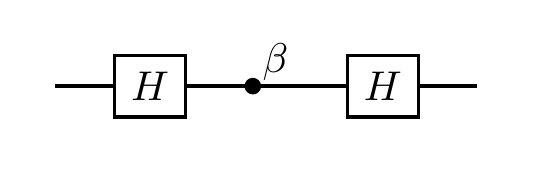
\begin{tikzpicture}
\node[scale=1.5] {
\begin{quantikz}
& \gate{H} & \phase{\beta} & \gate{H} & \qw
\end{quantikz}
};
\end{tikzpicture}
\end{center}
\tcblower
\begin{lstlisting}
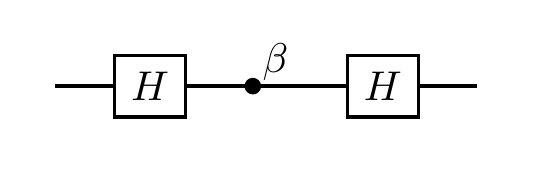
\begin{tikzpicture}
\node[scale=1.5] {
\begin{quantikz}
& \gate{H} & \phase{\beta} & \gate{H} & \qw
\end{quantikz}
};
\end{tikzpicture}
\end{lstlisting}
\end{Code}
It's also possible to rescale to a fixed width, so long as you declare the \verb!adjustbox! package in the document preamble.
\begin{Code}
\begin{center}
\begin{adjustbox}{width=0.8\textwidth}
\begin{quantikz}
& \gate{H} & \phase{\beta} & \gate{H} & \qw
\end{quantikz}
\end{adjustbox}
\end{center}
\tcblower
\begin{lstlisting}
\begin{adjustbox}{width=0.8\textwidth}
\begin{quantikz}
& \gate{H} & \phase{\beta} & \gate{H} & \qw
\end{quantikz}
\end{adjustbox}
\end{lstlisting}
\end{Code}


\section{Typesetting}

\subsection{Global Styling}

Global properties that affect all circuit elements of a given type can be affected through \verb!tikzset!.
\begin{Code}
\begin{center}
\tikzset{
	operator/.append style={fill=red!20},
	my label/.append style={above right,xshift=0.3cm},
	phase label/.append style={label position=above}
}
\begin{quantikz}
& \gate{H} & \phase{\beta} & \gate{H} & \qw & \meter{$\ket{\pm}$}
\end{quantikz}
\end{center}
\tcblower
\begin{lstlisting}
\tikzset{
  operator/.append style={fill=red!20},
  my label/.append style={above right,xshift=0.3cm},
  phase label/.append style={label position=above}
}
\begin{quantikz}
& \gate{H} & \phase{\beta} & \gate{H} & \qw & \meter{$\ket{\pm}$}
\end{quantikz}
\end{lstlisting}
\end{Code}
The global styles are:
\begin{center}
\begin{tabular}{c|c}
Style Name & Affected Command(s)	\\
\hline
operator & \verb!\gate!	\\
meter & \verb!\meter! \\
slice & \verb!\slice! \\
wave & \verb!\wave! \\
leftinternal	& \verb!\gateinput! \\
rightinternal	& \verb!\gateoutput! \\
dm & left braces (\verb!\gateoutput!,\verb!\lstick!) \\
dd & right braces (\verb!\gateinput!,\verb!\rstick!) \\
phase & \verb!\phase!, \verb!\control! \\
ophase & \verb!\ophase!, \verb!\ocontrol! \\
circlewc & \verb!\targ! \\
crossx2 & \verb!\swap!,\verb!\targX! \\
my label & measurement bases in \verb!\meter! \\
phase label & phases in \verb!\phase! \\
gg label & main gate label in \verb!\gate! \\
group label & label in \verb!\gategroup!
\end{tabular}
\end{center}

There are two keys that change styles globally: `thin lines' to make the lines thin, more in keeping with what QCircuit produced
\begin{Code}
\begin{center}
\begin{quantikz}[thin lines]
& \ctrl{1} & \qw & \ctrl{1} & \qw & \qw \\
& \targ{} & \gate{R_z(-\theta/2)} & \targ{} & \gate{R_z(\theta/2)} & \meter{}
\end{quantikz}
\end{center}
\tcblower
\begin{lstlisting}
\begin{quantikz}[thin lines]
& \ctrl{1} & \qw & \ctrl{1} & \qw & \qw \\
& \targ{} & \gate{R_z(-\theta/2)} & \targ{} 
  & \gate{R_z(\theta/2)} & \meter{}
\end{quantikz}
\end{lstlisting}
\end{Code}
\noindent and `transparent', should you want the background of all the gates to be transparent:
\begin{Code}
\begin{center}
\begin{quantikz}[transparent]
& \ctrl{1} & \qw & \ctrl{1} & \qw & \qw \\
& \targ{} & \gate{R_z(-\theta/2)} & \targ{} & \gate{R_z(\theta/2)} & \meter{}
\end{quantikz}
\end{center}
\tcblower
\begin{lstlisting}
\begin{quantikz}[transparent]
& \ctrl{1} & \qw & \ctrl{1} & \qw & \qw \\
& \targ{} & \gate{R_z(-\theta/2)} & \targ{} 
  & \gate{R_z(\theta/2)} & \meter{}
\end{quantikz}
\end{lstlisting}
\end{Code}

One place where this might be useful is as a ``pass-through'' on a gate, such as 
\begin{Code}
\begin{center}
\begin{quantikz}[transparent]
& \gate[2]{J_{12}} & \gate[3,label style={yshift=0.2cm}]{J_{13}} & \qw & \qw	\\
& & \linethrough &\gate[2]{J_{23}} & \qw \\
& \qw &&& \qw
\end{quantikz}
\end{center}
\tcblower
\begin{lstlisting}
\begin{quantikz}[transparent]
& \gate[2]{J_{12}} & \gate[3,label style={yshift=0.2cm}]{J_{13}} & \qw & \qw	\\
& & \linethrough &\gate[2]{J_{23}} & \qw \\
& \qw &&& \qw
\end{quantikz}
\end{lstlisting}
\end{Code}
While the \verb!\linethrough! would normally be hidden behind the gate, making the gate transparent leaves the line visible. Then one just has to move the $J_{13}$ label (see next section).

\subsection{Per-Gate Styling}

Individual gates can be modified using optional arguments of the calling function. 
\begin{Code}
\begin{center}
\begin{quantikz}
& \gate[style={fill=red!20},label style=cyan]{H} & \phase[green,label position=above]{\beta} & \gate{H} & \qw & \meter[draw=blue]{$\ket{\pm}$}
\end{quantikz}
\end{center}
\tcblower
\begin{lstlisting}
\begin{quantikz}
& \gate[style={fill=red!20},label style=cyan]{H} 
  & \phase[green,label position=above]{\beta} 
  & \gate{H} & \qw & \meter[draw=blue]{$\ket{\pm}$}
\end{quantikz}
\end{lstlisting}
\end{Code}
The specific syntax varies a little depending on the type of gate
\begin{center}
\begin{tabular}{p{0.4\textwidth}|p{0.4\textwidth}}
gates that don't accept formatting parameters & \verb!\qw!,\verb!\vqw!,\verb!\qwbundle!,\verb!\cw!,\verb!\vcw!,\verb!\cwbend!,\verb!\push!	\\
\hline
gates that accept tikz node formatting keys directly in optional argument & \verb!\phase!, \verb!\control!, \verb!\ocontrol!, \verb!\targ!, \verb!\targX!, \verb!\trash!, \verb!\meter!, \verb!\meterD!, \verb!\measure!, \verb!\measuretab!, \verb!\wave! \\
\hline
gates that accept node formatting keys as \verb!label style! key in optional argument & \verb!\gate!, \verb!\slice!, \verb!\lstick!, \verb!\rstick!, \verb!\gategroup!, \verb!\gateinput!, \verb!\gateoutput!
\end{tabular}
\end{center}
Those that accept the \verb!label style! key also accept a second key for formatting other elements of the display
\begin{center}
\begin{tabular}{c|cc}
\verb!\gate!,\verb!\gategroup! & \verb!style! & styles the box	\\
\verb!\slice! & \verb!style! & styles the line\\
\verb!\lstick!,\verb!\rstick!,\verb!\gateinput!,\verb!\gateoutput! & \verb!braces! & styles the brace
\end{tabular}
\end{center}
If you want to input several styling parameters with one of these keys, just group them together in a set of curly braces, \{\}. Typical styling parameters include \verb!draw=! specifying line colour, \verb!fill=!, specifying fill colour, \verb!inner xsep=! and \verb!inner ysep=! specifying horizontal and vertical margins respectively, \verb!xshift=! and \verb!yshift=! for adjusting horizontal and vertical positioning. Beyond that, the \href{http://mirrors.ctan.org/graphics/pgf/base/doc/pgfmanual.pdf}{tikz manual} is your friend!

This styling is really quite flexible, as we can override the default shapes with anything that we want:
\begin{Code}
\begin{center}
\tikzset{
	group-1-5/.append style={starburst,fill=yellow,draw=red,line width=2pt,inner ysep=-15pt}
}
\begin{quantikz}[row sep=0.3cm,column sep=0.3cm]%
& \gate{H} & \ctrl{2}& \qw & \gate[3,style={starburst,fill=yellow,draw=red,line width=2pt,inner xsep=-4pt,inner ysep=-5pt},label style=cyan]{\text{noise}} & \ctrl{3} & \qw  & \qw & \qw\\
\lstick{$\ket{0}$} & \qw & \targ{} & \qw & \qw & \qw & \ctrl{3} & \qw & \qw \\
\lstick{$\ket{0}$} & \qw & \targ{}& \qw & \qw & \qw & \qw & \ctrl{2} & \qw\\
&&&&\lstick{$\ket{0}$} & \targ{} & \targ{} & \qw & \meter{} \\
&&&&\lstick{$\ket{0}$} & \qw & \targ{} & \targ{} & \meter[draw=blue]{} 
\end{quantikz}
\end{center}
\tcblower
\begin{lstlisting}
\begin{quantikz}[row sep=0.3cm,column sep=0.3cm]%
& \gate{H} & \ctrl{2}& \qw & 
  \gate[3,style={starburst,fill=yellow,draw=red,line width=2pt,inner xsep=-4pt,inner ysep=-5pt},
    label style=cyan]{\text{noise}} & \ctrl{3} & \qw  & \qw& \qw\\
\lstick{$\ket{0}$} & \qw & \targ{} & \qw & \qw & \qw & \ctrl{3} & \qw & \qw \\
\lstick{$\ket{0}$} & \qw & \targ{}& \qw & \qw & \qw & \qw & \ctrl{2} & \qw\\
&&&&\lstick{$\ket{0}$} & \targ{} & \targ{} & \qw & \meter{} \\
&&&&\lstick{$\ket{0}$} & \qw & \targ{} & \targ{} & \meter[draw=blue]{} 
\end{quantikz}
\end{lstlisting}
\end{Code}
% We can also supplement with standard tikz commands by using the `execute at end picture' key. The cells of the matrix contain nodes called \verb!\tikzcdmatrixname-i-j!, where i is the row number and j is the column number. Thus,
% \begin{Code}
% \begin{center}
% \begin{quantikz}[row sep=0.3cm,column sep=0.3cm,execute at end picture={
% 	\node [fit=(\tikzcdmatrixname-1-6)(\tikzcdmatrixname-4-6)(\tikzcdmatrixname-5-9),draw,dashed,inner sep=4pt,label={[yshift=0.3cm]above:syndrome extraction}] {};
% }]
% & \gate{H} & \ctrl{2}& \qw & \gate[3,style={starburst,fill=yellow,draw=red,line width=2pt,inner xsep=-4pt,inner ysep=-5pt}]{\text{noise}} & \ctrl{3} & \qw  & \qw& \qw\\
% \lstick{$\ket{0}$} & \qw & \targ{} & \qw & \qw & \qw & \ctrl{3} & \qw & \qw \\
% \lstick{$\ket{0}$} & \qw & \targ{}& \qw & \qw & \qw & \qw & \ctrl{2} & \qw\\
% &&&&\lstick{$\ket{0}$} & \targ{} & \targ{} & \qw & \meter{} \\
% &&&&\lstick{$\ket{0}$} & \qw & \targ{} & \targ{} & \meter{} 
% \end{quantikz}
% \end{center}
% \tcblower
% \begin{lstlisting}
% \begin{quantikz}[row sep=0.3cm,column sep=0.3cm,execute at end picture={
% 	\node [fit=(\tikzcdmatrixname-1-6)(\tikzcdmatrixname-4-6)(\tikzcdmatrixname-5-9),draw,dashed,inner sep=4pt,label={[yshift=0.3cm]above:syndrome extraction}] {};
% }]
% & \gate{H} & \ctrl{2}& \qw & \gate[3,style={starburst,fill=yellow,draw=red,line width=2pt,inner xsep=-4pt,inner ysep=-5pt}]{\text{noise}} & \ctrl{3} & \qw  & \qw& \qw\\
% \lstick{$\ket{0}$} & \qw & \targ{} & \qw & \qw & \qw & \ctrl{3} & \qw & \qw \\
% \lstick{$\ket{0}$} & \qw & \targ{}& \qw & \qw & \qw & \qw & \ctrl{2} & \qw\\
% &&&&\lstick{$\ket{0}$} & \targ{} & \targ{} & \qw & \meter{} \\
% &&&&\lstick{$\ket{0}$} & \qw & \targ{} & \targ{} & \meter{} 
% \end{quantikz}
% \end{lstlisting}
% \end{Code}

\subsection{Boxing/Highlighting Parts of a Circuit}\label{sec:boxing}

It is often useful to highlight parts of a circuit. We do this with the \verb!\gategroup! command. The optional parameters \verb!wires! (again, the default) and \verb!steps! specify the number of rows and columns that the group spans respectively. The mandatory argument is the label for the box (although this can be empty). The top-left corner of the box coincides with the cell in which the command is placed.
\begin{Code}
\begin{center}
\begin{quantikz}
& \gate{H} & \ctrl{1} & \gate{H}\gategroup[wires=2,steps=3,style={inner sep=6pt}]{reversed c-{\sc not}} & \ctrl{1} & \gate{H} & \ctrl{1} & \qw & \qw \\
& \qw & \targ{} & \gate{H} & \targ{} & \gate{H} & \targ{} & \gate{H} & \qw
\end{quantikz}
\end{center}
\tcblower
\begin{lstlisting}
\begin{quantikz}
& \gate{H} & \ctrl{1} & \gate{H}\gategroup[wires=2,steps=3,style={inner sep=6pt}]{reversed c-{\sc not}} & \ctrl{1} & \gate{H} & \ctrl{1} & \qw & \qw \\
& \qw & \targ{} & \gate{H} & \targ{} & \gate{H} & \targ{} & \gate{H} & \qw
\end{quantikz}
\end{lstlisting}
\end{Code}
By default, this box is drawn on top of the circuit itself. If you want it to be behind (for example, should you want it to have a background colour), then use the \verb!background! option.
\begin{Code}
\begin{center}
\begin{quantikz}
& \gate{H} & \ctrl{1}\gategroup[2,steps=3,style={dashed,rounded corners,fill=blue!20, inner xsep=2pt},background]{{\sc swap}} & \targ{} & \ctrl{1} & \qw & \qw \\
& \qw & \targ{} & \ctrl{-1} & \targ{} & \gate{H} & \qw
\end{quantikz}
\end{center}
\tcblower
\begin{lstlisting}
\begin{quantikz}
& \gate{H} & \ctrl{1}\gategroup[2,steps=3,style={dashed,rounded corners,fill=blue!20, inner xsep=2pt},background]{{\sc swap}} & \targ{} & \ctrl{1} & \qw & \qw \\
& \qw & \targ{} & \ctrl{-1} & \targ{} & \gate{H} & \qw
\end{quantikz}
\end{lstlisting}
\end{Code}
The \verb!label style! key can be used to tune the label's properties, including positioning. For example,
\begin{Code}
\begin{center}
\begin{quantikz}
& \gate{H} & \ctrl{1}\gategroup[2,steps=3,style={dashed,rounded corners,fill=blue!20, inner xsep=2pt},background,label style={label position=below,anchor=north,yshift=-0.2cm}]{{\sc swap}} & \targ{} & \ctrl{1} & \qw & \qw \\
& \qw & \targ{} & \ctrl{-1} & \targ{} & \gate{H} & \qw
\end{quantikz}
\end{center}
\tcblower
\begin{lstlisting}
\begin{quantikz}
& \gate{H} & \ctrl{1}\gategroup[2,steps=3,style={dashed,rounded corners,fill=blue!20, inner xsep=2pt},background,label style={label position=below,anchor=north,yshift=-0.2cm}]{{\sc swap}} & \targ{} & \ctrl{1} & \qw & \qw \\
& \qw & \targ{} & \ctrl{-1} & \targ{} & \gate{H} & \qw
\end{quantikz}
\end{lstlisting}
\end{Code}
Note that it is often good to use \verb!anchor=mid! for label anchors because if you have multiple labels, this will help get them horizontally aligned. It just means you have to use some \verb!yshift! to move the label off the border around the gategroup.


At this point, we mention an extra option for the gate command. The \verb!swap! keyword turns the gate into a variant of a {\sc swap} gate which explicitly shows the wires (the \verb!wires! setting is fixed to 2, overriding any value you might supply).
\begin{Code}
\begin{center}
\begin{quantikz}
& \gate{H} & \gate[swap]{} & \qw & \qw \\
& \qw &  & \gate{H} & \qw
\end{quantikz}
\end{center}
\tcblower
\begin{lstlisting}
\begin{quantikz}
& \gate{H} & \gate[swap]{} & \qw & \qw \\
& \qw &  & \gate{H} & \qw
\end{quantikz}
\end{lstlisting}
\end{Code}
%\noindent Here the \texttt{fullwidth} command is helpful for getting the symmetry of the swap gate correct in terms of how much goes above the top wire, and how much below the bottom wire.
\section{Otherwise Undocumented Features}
A wave for separating rows. Do we really need this? Perhaps not, but it's fun!
\begin{Code}
\begin{center}
\begin{quantikz}
& \gate{H} & \ctrl{3} & \ \ldots\ \qw & \qw & \gate{H} & \qw \\
\wave&&&&&&\\
& \gate{H} & \qw & \ \ldots\ \qw & \ctrl{1} & \gate{H} & \qw \\
& \qw & \gate{U} & \ \ldots\ \qw & \gate{U^k} & \qw & \qw
\end{quantikz}
\end{center}
\tcblower
\begin{lstlisting}
\begin{quantikz}
& \gate{H} & \ctrl{3} & \ \ldots\ \qw & \qw & \gate{H} & \qw \\
\wave&&&&&&\\
& \gate{H} & \qw & \ \ldots\ \qw & \ctrl{1} & \gate{H} & \qw \\
& \qw & \gate{U} & \ \ldots\ \qw & \gate{U^k} & \qw
\end{quantikz}
\end{lstlisting}
\end{Code}


Creating an ebit. The single parameter is whatever text you want. The first optional parameter specifies the angle of the initial line relative to the vertical, which defaults to -45. The second optional parameter gives stylings for the text label.
\begin{Code}
\begin{center}
\begin{tikzcd}
& \makeebit[-60][blue]{test} & \qw & \qw \\
 & & \qw & \qw
\end{tikzcd}
\end{center}
\tcblower
\begin{lstlisting}
\begin{tikzcd}
& \makeebit[-60][blue]{test} & \qw & \qw \\
 & & \qw & \qw
\end{tikzcd}
\end{lstlisting}
\end{Code}

\section{Converting from QCircuit}

I've updated all of my existing teaching materials from QCircuit to Quantikz with very little trouble. There are a few standard replacements:
\begin{center}
\begin{tabular}{c|c}
QCircuit notation & Quantikz notation \\
\hline
\verb!\QCircuit @C=n @R=m {#}! & \verb!\begin{quantikz}[row sep=m,col sep=n]#\end{quantikz}!	\\
\verb!\multigate{n}! & \verb!\gate[n+1]!	\\
\verb!\targ! & \verb!\targ{}! \\
\verb!\control! & \verb!\control{}! \\
\verb!\meter! & \verb!\meter{}! \\
\verb!\measureD! & \verb!\meterD{}! \\
\end{tabular}
\end{center}
Updating the \verb!\gategroup! command requires a little more care since the first two arguments have to be removed, and the command placed in the correct cell, at which point \verb!\gategroup{i}{j}{k}{l}{m}! becomes \verb!\gategroup[wires=k+1-i,steps=l+1-j]!. My primary use of gategroup was to achieve the effect now achieved with \verb!\lstick[k+1-i]!.

It should not be necessary to use \verb!\ghost! commands in the way they were used in QCircuit. The \verb!\cghost! and \verb!\nghost! commands have been replaced by option keys for the gate command, \verb!cwires! and \verb!nwires! respectively.

\section{Troubleshooting}\label{sec:trouble}
\begin{itemize}
\item Have you checked that all commands that need them are followed by an empty argument, \{\}? Things like \verb!meter!, \verb!\control! (basically, those that can accept an optional styling parameter) look like they don't take any parameters, but they have to be followed by the pair of braces or you'll get very odd effects.
\item If you get a whole bunch of unexpected text in one of your cells instead of a gate, make sure that the gate command is the first command in the cell, and that other commands (such as \verb!\qwbundle!) appear after.
\item If you're getting errors about cells not being found (and especially if you're doing any slicing), check that your last row doesn't end with \textbackslash\textbackslash, and make sure that your last row contains as many cells (even if they're empty) as there are columns in the circuit.
\item If you are trying to typeset your circuit inside some sort of tabular or align environment and are getting an error ``single ampersand used with wrong catcode'', trying adding the \verb![ampersand replacement=\&]! option to tikzcd, and instead of separating every cell by \&, use \textbackslash\&. This can also be useful if you want to insert a normal matrix as a gate
\begin{Code}
\begin{center}
\begin{quantikz}[ampersand replacement=\&]
\lstick{$\ket{0}$} \& \gate{\left(\begin{array}{cc} \alpha & \beta \\ \beta & -\alpha \end{array}\right)} \& \ctrl{1} \& \gate{U_1} \& \qw \\
\lstick{$\ket{0}$} \& \qw \& \targ{} \& \gate{U_2} \& \qw
\end{quantikz}
\end{center}
\tcblower
\begin{lstlisting}
\begin{quantikz}[ampersand replacement=\&]
\lstick{$\ket{0}$} \& \gate{\left(\begin{array}{cc} \alpha & \beta \\ \beta & -\alpha \end{array}\right)} \& \ctrl{1} \& \gate{U_1} \& \qw \\
\lstick{$\ket{0}$} \& \qw \& \targ{} \& \gate{U_2} \& \qw
\end{quantikz}
\end{lstlisting}
\end{Code}
Beamer is particularly annoying with doing this. It probably helps to issue a global command
\begin{lstlisting}
\tikzcdset{
	every matrix/.style={ampersand replacement=\&}
}
\end{lstlisting}
somewhere in your document preamble. The tikzcd manual suggests another possible strategy, but I haven't had much success with it.
\item If you're using a circuit diagram inside an \texttt{align} environment, the \texttt{tikzcd} environment works better than \texttt{quantikz}. You may also need to use the ampersand replacement strategy.
\item If you have a \verb!\cwbend! in the bottom right cell of the matrix, sometimes you get an error (I have no understanding of why). Add an extra \& after, and all seems to be well.
\item If you're using transparency, and the width of gates seems to be greater than you expected, it may be worthwhile removing the .aux file and recompiling. If your tex editor isn't good at resetting the .aux file, the system may be remembering older widths.
\item The code provides definitions for \verb!\bra!, \verb!\ket!, \verb!\proj!, \verb!\braket!. If you don't like them, just define your own versions \emph{before} you load the quantikz library.
\item Package load order: I've had reports that if you load certain packages in the wrong order it can create weird errors. For example, if you load the package cleveref after quantikz, and then use a split environment, it can lead to the error ``Only one \# is allowed per tab.''. Change the load order and it goes away. I have no idea why this happens.
\end{itemize}

For any bug reports (please make sure you've checked the above list first!) or feature requests, please contact alastair.kay@rhul.ac.uk.

\section{Citation}

If you found this package useful, please consider citing the arXiv version of this document, arXiv:1809.03842.


\end{document} 